\section{Evaluation}\label{sec:evaluation}

To evaluate the performances of our approach, we first evaluate its  raw speed with a test class that we made for the occasion. We also ran two series of tests: we first tested all classes in \texttt{java.lang} $10^{6}$ times each. We also tested a package from iText\footnote{http://www.lowagie.com/iText/ downloaded Sep. 1, 2009} a well known library -- 1,969,220 downloads on SourceForge\footnote{http://sourceforge.net/projects/itext/}, $84\%$ positive advices, activity of $99.85\%$ -- for manipulating PDF documents in Java. 

All tests were run using a MacBook Pro 2.53 GHz Intel Core 2 Duo, 4GB of 1067 MHz DDR3 of RAM, under MacOSX with the Java(TM) SE Runtime Environment (build 1.6.0\_15-b03-219) -- with default value of 64MB of RAM reserved. 

\subsection{Performances}

To test raw performances of YETI, we made two small classes -- \texttt{Perf} and \texttt{Perf1} shown in Figure~\ref{fig:perf} -- that we tested 30 times each with one million tests. Results are presented in Figures~\ref{fig:perfDriver} and~\ref{fig:perfValue}.

\begin{figure}[ht!]
{\small
\begin{verbatim}
public class Perf{
        int i=0;
        public void test(){
                i++;
        }
}
public class Perf1{
        public void test(int i){
                int j = i;
                i++;
                assert(i>j);
        }
}
\end{verbatim}
}
\caption{Classes used for measuring performances.}\label{fig:perf}
\end{figure}

While \texttt{Perf} does not exhibit failures, \texttt{Perf1} exhibits failures when \texttt{i} is equal to \texttt{MAX\_INT} if assertions are enabled (which we chose to do in this test).

\begin{figure}[ht!]
\begin{center}
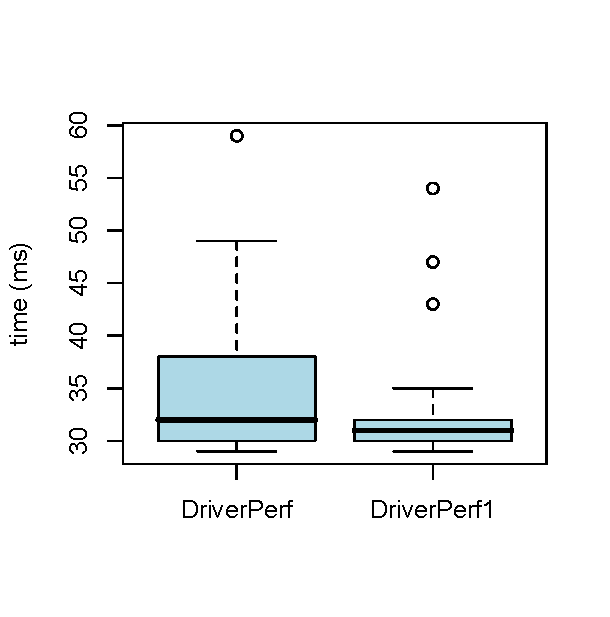
\includegraphics[width=6cm]{images/DriverWhiskers.pdf}
\end{center}
\caption{Evaluation of the code of Perf and Perf1 with an external driver.}\label{fig:perfDriver}
\end{figure}

To make sure that we only tested the overhead of the infrastructure, we also made one million calls on each of the methods from another program. Figure~\ref{fig:perfDriver} shows box and whisker plots for the two raw tests.

\begin{figure}[ht!]
\begin{center}
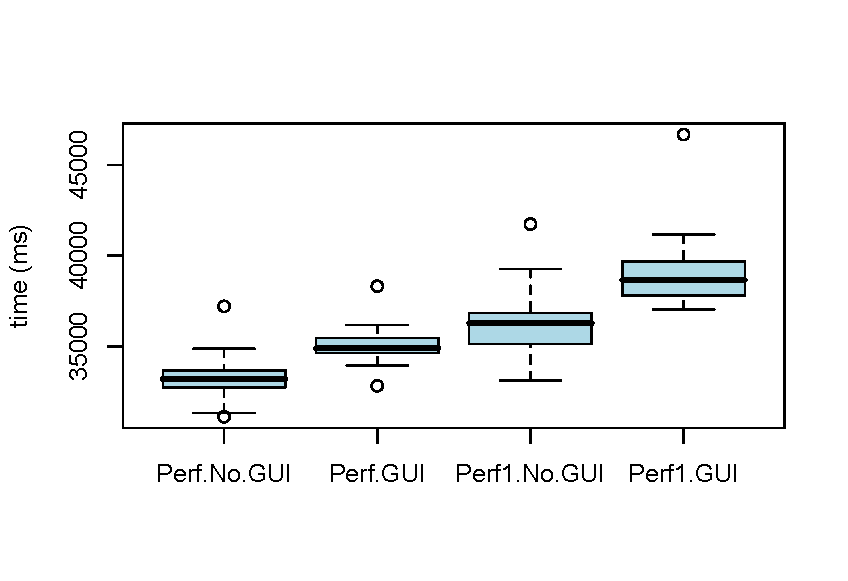
\includegraphics[width=8cm]{images/PerfWhiskers.pdf}
\end{center}
\caption{Evaluation of the code of Perf and Perf1 tested by YETI, with and without GUI. Averages: 33200(Perf No GUI), 35018(Perf GUI), 36103(Perf1 No GUI), 39021(Perf1 GUI)}\label{fig:perfValue}
\end{figure}

Figure~\ref{fig:perfValue} shows box and whisker plots for 30 YETI testing sessions of one million tests made on \texttt{Perf} and \texttt{Perf1}, both with and without the GUI. We can see that there is a slowdown of more than a factor 1000 over the direct invocation. The GUI also incurs respectively a $5.5\%$ and $8.1\%$ overhead.

Eventually, even over long running sessions (when logs are not stored within YETI) the number of routine calls effected, grows linearly with time as shown in Figure~\ref{fig:string} for a 50 minute session testing \texttt{java.lang.String}.

\begin{figure}[h!]
\begin{center}
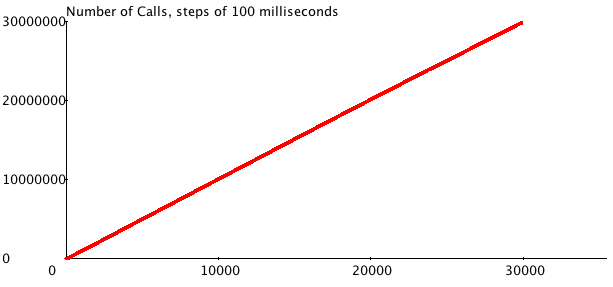
\includegraphics[width=\columnwidth]{images/Ncalls.png}
\end{center}
\caption{Number of calls over time while testing \texttt{java.lang.String}}\label{fig:string}
\end{figure}



\subsection{Testing \texttt{java.lang}}

\begin{table*}[ht!]
\caption{Results of testing java.lang}\label{tab:javalang}
\scalebox{.9}{\begin{minipage}{\textwidth}
{\small
\begin{center}
\begin{tabular}{l c c c c c c c c}
\hline
&\begin{sideways}Total throwables\end{sideways}&\begin{sideways}Faults\end{sideways}&\begin{sideways}NullPointer\end{sideways}&\begin{sideways}NoClassDefFoundError\end{sideways}&\begin{sideways}IndexOutOfBounds\end{sideways}&\begin{sideways}AssertionError\end{sideways}&\begin{sideways}IllegalArgument\end{sideways}\\
\hline
Boolean &1&0&0&&&&\\
Byte &2&2&2&&&&\\
Character &33&1&1&&&&\\
Character.Subset &0&0&&&&&\\
Character.UnicodeBlock &2&0&&&&&\\
Class &13&3&3&&&&\\
ClassLoader &10&10&8&2&&&\\
Compiler &0&0&&&&&\\
Double &4&2&2&&&&\\
Enum &2&0&&&&&\\
Float &4&2&2&&&&\\
InheritableThreadLocal &0&&&&&&\\
Integer &2&2&2&&&&\\
Long &2&2&2&&&&\\
Math &0&&&&&&\\
Number &0&&&&&&\\
Object &0&&&&&&\\
Package &1&1&1&&&&\\
Process &0&&&&&&\\
ProcessBuilder &5&2&2&&&&\\
Runtime &2&0&&&&&\\
RuntimePermission &4&0&&&&&\\
SecurityManager &39&0&&&&&\\
Short &2&2&2&&&&\\
StackTraceElement &2&0&&&&&\\
StrictMath &0&&&&&&\\
String &87&5&&&2&3&\\
StringBuffer &57&3&&&2&&1\\
StringBuilder &36&2&1&&&&1\\
System &5&0&&&&&\\
Thread &18&5&5&&&&\\
ThreadGroup &4&0&&&&&\\
ThreadLocal &0&&&&&&\\
Throwable &2&0&&&&&\\
Void&0&&&&&&\\
EnumConstantNotPresentException&1&1&1&&&&\\
All Other Exceptions  &0&0&0&&&&\\
All Errors  &0&0&0&&&&\\
\hline
Total&340&45&34&2&4&3&2\\
\hline
Percentages&&&75.6&4.4&8.9&6.7&4.4\\
\hline
\end{tabular}
\end{center}
}
\end{minipage}}

\end{table*}

We tested all classes in \texttt{java.lang} with YETI. For each class we requested $1,000,000$ tests. Except for a couple of classes that were too memory intensive -- such as \texttt{StringBuffer} -- that we tested with $100,000$ tests only.
Table~\ref{tab:javalang} shows our results. The first column of numbers indicates the total number of
throwables that the tests triggered. We then classified each throwable as either a fault or not. This is due to programmers not necessarily declaring runtime exceptions but rather indicating in the documentation that these exceptions are normal. For throwables that where not ruled out, 
we then classify them by column. Note that the documentation of certain classes states up front that
some kind of exceptions are to be expected -- for example \texttt{NullPointerException} in \texttt{String}.
Other classes declare all runtime exceptions. This indicates that several teams actually collaborated to make this API. 

The small number of faults other than \texttt{NullPointerException}s, shows the overall quality of \texttt{java.lang} in terms of API and implementation. Most exceptions seem indeed to be omitted in the documentation rather than real bugs in the system.

It is however compelling to see that YETI can actually uncover 45 faults in a library as used and tested as \texttt{java.lang}. 
While these faults are real, it is to be noted that we only uncover runtime faults (runtime exceptions and errors) and it has no knowledge of methods that should be called in specific orders.
Faults resulting from the misuse of such methods are still reported as faults by the TOOL.
To obtain more data to assess how useful YETI would be for regular developers, we present similar results for a regular open source project in the next section.



\subsection{Testing \texttt{com.lowagie.text} from iText}
\begin{table*}[ht!]
\caption{Results of testing com.lowagie.text}\label{tab:comlowagietext}
\begin{minipage}{\textwidth}
{\small
\begin{center}
\begin{tabular}{l c c c c c c c c c c c c c c c}
\hline
&\begin{sideways}Total throwables\end{sideways}&\begin{sideways}Number of Faults\end{sideways}&\begin{sideways}NullPointer\end{sideways}&\begin{sideways}IndexOutOfBounds\end{sideways}&\begin{sideways}NumberFormatException\end{sideways}&\begin{sideways}IllegalArgumentException\end{sideways}&\begin{sideways}No class def found\end{sideways}&\begin{sideways}ClassCast\end{sideways}&\begin{sideways}IllegalState\end{sideways}&\begin{sideways}NegativeArraySize\end{sideways}&\begin{sideways}Runtime\end{sideways}&\begin{sideways}ArrayStore\end{sideways}&\begin{sideways}StackOverflow\end{sideways}&\begin{sideways}Project-defined\end{sideways}\\
\hline
Total&138&120&38&20&2&5&6&4&1&6&1&2&2&33\\
\hline
Percentage&&86.2&31.9&16.8&1.7&4.2&5.0&3.4&0.8&5.0&0.8&1.7&1.7&27.7\\
\hline
\end{tabular}
\end{center}
}
\end{minipage}
\end{table*}

In order to have a more representative project for end-users, we tested the package \texttt{com.lowagie.text} from iText. Table~\ref{tab:comlowagietext} shows the aggregated results of the tests. Because this package is quite time intensive to test, we decided to test all classes in the package at the same time for only a $100000$ tests. The testing session lasted for 15 minutes and output 138 unique failures. Comparatively to the previous section, the code almost did not declare any runtime exception. Only five classes --~\texttt{Cell}, \texttt{MarkedSection}, \texttt{Phrase}, \texttt{RectangleReadOnly}, and \texttt{Section}~-- did it in an informal way. 

It is worth noting that two classes --~\texttt{RectangleReadOnly}  and \texttt{Document}~-- exhibit a high number of project-defined errors. We investigated and found out that these two classes have poor documentation rather than poor code. This is to be expected in a free open source project as the code often serves as documentation.

\subsection{Reporting in Real-Time}

Other random testing tools do not include any way of interacting with the infrastructure in real-time.
YETI allows it and it benefits test engineers because they can adapt the testing process to fit their needs. In this subsection, we show two scenarios where having real-time reporting in YETI allows test engineers to adapt and circumvent issues.

\paragraph{Using results from other techniques}
\begin{figure}[ht!]
{\small
\begin{verbatim}
// A class where random does not find 
// the bug unless very lucky
public class MyClass{
   public int div(int i){
      return i/(4556767-i);
   }
}
// Helper class to generate the interesting 
// value 4556767 in priority
public class HelpMyClass {
   public static int value(){
     return 4556767; 
   }
}
\end{verbatim}
}
\caption{A class to test.}\label{fig:myClass}
\end{figure}

Figure~\ref{fig:myClass} shows the code of \texttt{MyClass}, a class that only contains a method that calculates $i/(4556767-i)$ ($i$ being its argument). Obviously, passing $4556767$ as an argument will lead to a failure. When using a black-box random testing approach, for the tool to test that method with $4556767$ 
requires it to be lucky or to wait for a potentially long time for the testing to perform. 
A more realistic approach is that users might launch the testing session and then, because they do not find a fault at the beginning of the session, decide to find values from the code or the documentation. In our case a software tester might then create the class \texttt{HelpMyClass} (see Figure~\ref{fig:myClass}) that contains a method returning that value and load it at runtime.

\begin{figure}[h!]
\begin{center}
\includegraphics[width=\columnwidth]{images/HelpMyClass.png}
\end{center}
\caption{Faults evolution when introducing HelpMyClass at 56s, \texttt{div} had been called $3\times10^{5}$ times out of $2\times10^{6}$ total calls.}\label{fig:helpmyclass}
\end{figure}

Figure~\ref{fig:helpmyclass} shows that the fault is then found immediately after the test engineer loads \texttt{HelpMyClass} into the system (56s after the beginning of testing).

\paragraph{Testing untested methods and adapting the strategy at runtime}

One of the visible issues in Figure~\ref{fig:gui} is that the method \texttt{contentEquals} from \texttt{String} is not tested by YETI. The reason is that it uses instances of the class \texttt{StringBuffer} and even if the JVM knows it, YETI does not. The reason is that, for performances reasons, YETI does not load the whole transitive closure of types used in the tested program. The natural reaction in such a case is for the test engineer to add the module (load the class using the button in the lower-left part of the GUI). 

The issue is that \texttt{StringBuffer} is a buffer that can be initialized with a pre-defined capacity (an \texttt{int}). If numerous instances are initialized using large values, then the performances drop due to the large amount of memory needed by the JVM. A recovery strategy is to limit the number of instances per type.

\begin{figure*}[ht!]
\begin{center}
\includegraphics[width=.75\textwidth]{images/StringBuffer.png}
\end{center}
\caption{Testing \texttt{String}, adding \texttt{StringBuffer}, and then reducing the number of instances per type (in this case 2).}\label{fig:StringBuffer}
\end{figure*}

Figure~\ref{fig:StringBuffer} presents the graphs obtained in such a scenario. It is clearly visible in the figure that introducing \texttt{StringBuffer} has a positive impact on the number of faults. It also impacts however the performances. By reducing the number of instances per type we then improve the situation, which also allows YETI to find more faults.
